\chapter{Projective planes}

Some may already encountered the projective planes or at least their finite versions. In this chapter we will recall the definition and also some properties they have.

\section{Basics}

\begin{defn}
	Projective plane is hypergraf $(X, \mathcal{M})$ such that
	
	\begin{enumerate}
		\item every two (different) edges (or lines) intersect in exactly 1 point,
		\label{projective-plane-1st}
		\item for every 2 (distinct) points there exist exactly one edge containing them, \label{projective-plane-2nd}
		\item there are four points so no 3 of them lies on same edge. \label{projective-plane-3rd}
	\end{enumerate}
\end{defn}

\noindent One of the most well known finite projective plane is Fano plane, which can be seen on a picture \ref{fano-plane}.

\begin{figure}[!h]\centering
	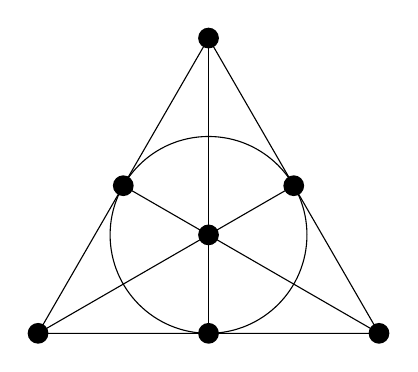
\begin{tikzpicture}[scale=2.5]
		\draw (0,0) circle (0.5);
		\draw (90:1) -- (-30:1)--(210:1)--cycle;
		\draw (90:1)--(0,0);
		\draw (210:1)--(0,0);
		\draw (-30:1)--(0,0);
		\draw (30:0.5)--(0,0);
		\draw (150:0.5)--(0,0);
		\draw (270:0.5)--(0,0);
		\fill (-0.866,-0.5) circle (1.5pt);
		\fill (0.866,-0.5) circle (1.5pt);
		\fill (0,-0.5) circle (1.5pt);
		\fill (0,1) circle (1.5pt);
		\fill (0,0) circle (1.5pt);
		\fill (0.433,0.25) circle (1.5pt);
		\fill (-0.433,0.25) circle (1.5pt);
	\end{tikzpicture}
	\caption{Fano plane.}
	\label{fano-plane}
\end{figure}

\begin{example}
	Now what about euclidean space $\R^2$? We can obviously see that part \ref{projective-plane-3rd} is satisfied, and also the property \ref{projective-plane-2nd}. Only for the very first one \ref{projective-plane-1st} we may encounter two lines which are parallel, hence they do not share any point. But we may establish an infinite point for which all such parallel lines in this direction go to. Therefore we must create a lot of infinite points, for every possible direction. But with such augmentation we have broken the property \ref{projective-plane-2nd} and so we need to add a line which goes through all infinite points.\label{r2-creation}
\end{example}

\section{Construction of projective planes}

As in the example \ref{r2-creation} shown before we will furthermore establish general technique to create a projective plane. Firstly in a geometric way and later on also in algebraic way.

Lets firstly start by taking 4 points, so we are trying to create a smallest possible finite projective plane. To fulfil all properties lets add few lines and end up with a box having two diagonals, see picture \ref{fano-plane-start}. Now we encounter the same problem as it was before, so we also add infinite points and extend the lines to them and also creating a line going through all of such infinite points. Note that \textit{parallel lines} now are those lines which don't cross each other in a point. With this procedure we get the following picture \ref{fano-plane-end} and we may see that it is indeed isomorphic to the well known Fano plane.

\begin{figure}[!h]\centering
	\begin{subfigure}{0.4\textwidth}\centering
		\begin{tikzpicture}[scale=1, l/.style = {line width=2pt},
			n/.style = {draw, circle, fill, inner sep=1.5pt},
			o/.style = {myorange},
			r/.style = {myred},
			b/.style = {myblue},
			g/.style = {mygreen},
			p/.style = {myviolet}]
			\node[n] (1) at (0,0) {};
			\node[n] (2) at (0,2) {};
			\node[n] (3) at (2,0) {};
			\node[n] (4) at (2,2) {};
			\draw[l,b] (1) to (2);
			\draw[l,b] (3) to (4);
			\draw[l,g] (2) to (3);
			\draw[l,g] (1) to (4);
			\draw[l,r] (1) to (3);
			\draw[l,r] (2) to (4);
		\end{tikzpicture}
		\caption{Starting box with 6 lines and 4 points.}
		\label{fano-plane-start}
	\end{subfigure}
	\begin{subfigure}{0.4\textwidth}\centering
		\begin{tikzpicture}[scale=1, l/.style = {line width=2pt},
			n/.style = {draw, circle, fill, inner sep=1.5pt},
			o/.style = {myorange},
			r/.style = {myred},
			b/.style = {myblue},
			g/.style = {mygreen},
			p/.style = {myviolet}]
			\node[n] (1) at (0,0) {};
			\node[n] (2) at (0,2) {};
			\node[n] (3) at (2,0) {};
			\node[n] (4) at (2,2) {};
			
			\node[n, r] (i1) at (3,1) {};
			\node[n, b] (i2) at (1,3) {};
			\node[n, g] (i3) at (1,-1) {};
			
			\draw[b, l] (1) to (2) to[out=90, in=180] (i2);
			\draw[b, l] (3) to (4) to[out=90, in=0] (i2);
			\draw[g, l] (2) to (3) to[out=270, in=0] (i3);
			\draw[g, l] (4) to (1) to[out=270, in=180] (i3);
			\draw[r,l] (1) to (3) to[out=0, in=270] (i1);
			\draw[r,l] (2) to (4) to[out=0, in=90] (i1);
			
			\draw[l,p] (0,-1) to (i3) to[out=0, in=270] (i1) to[out=90,in=0] (i2) to (0,3);
		\end{tikzpicture}
		\caption{Ending with 7 lines and 7 points.}
		\label{fano-plane-end}
	\end{subfigure}
	\caption{Generating smallest projective plane.}
\end{figure}

We can also apply to this to other starting points. We may see the result of applying to $3 \times 3$ grid of points and resulting in a projective plane depicted on picture \ref{3by3}.

\begin{figure}[!h]\centering
	\begin{subfigure}{0.4\textwidth}\centering
		\begin{tikzpicture}[scale=.6, l/.style = {line width=2pt},
			n/.style = {draw, circle, fill, inner sep=1.5pt},
			o/.style = {myorange},
			r/.style = {myred},
			b/.style = {myblue},
			g/.style = {mygreen},
			p/.style = {myviolet}]
			\foreach \j in {1,...,3} {
				\foreach \i in {1,...,3} {
					\node[n] (\j-\i) at (2*\j,2*\i) {};
				}
			}
			
			\draw[l,o] (1-1) to (1-2) to (1-3);
			\draw[l,o] (2-1) to (2-2) to (2-3);
			\draw[l,o] (3-1) to (3-2) to (3-3);
			
			\draw[l,b] (1-1) to (2-1) to (3-1);
			\draw[l,b] (1-2) to (2-2) to (3-2);
			\draw[l,b] (1-3) to (2-3) to (3-3);
			
			\draw[l,g] (1-1) to (2-2) to (3-3);
			\draw[l,g] (1-2) to (2-3) to[out=20,in=180] (6.5,6.5) to[out=0, in=0] (3-1);
			\draw[l,g] (1-3) to[out=200,in=180] (1.5,1.5) to[out=0,in=200] (2-1) to (3-2);
			
			\draw[l,r] (1-1) to[out=330,in=250] (6.5,1.5) to[out=70,in=330] (3-2) to (2-3);
			\draw[l,r] (3-3) to[out=120,in=0] (1.5,6.5) to[out=180,in=150] (1-2) to (2-1);
			\draw[l,r] (1-3) to (2-2) to (3-1);
		\end{tikzpicture}
		\caption{Starting $3 \times 3$ grid with lines and diagonals.}
	\end{subfigure}
	\begin{subfigure}{0.4\textwidth}\centering
		\begin{tikzpicture}[scale=.6, l/.style = {line width=2pt},
			n/.style = {draw, circle, fill, inner sep=1.5pt},
			o/.style = {myorange},
			r/.style = {myred},
			b/.style = {myblue},
			g/.style = {mygreen},
			p/.style = {myviolet}]
			\foreach \j in {1,...,3} {
				\foreach \i in {1,...,3} {
					\node[n] (\j-\i) at (2*\j,2*\i) {};
				}
			}
			
			\node[n,o] (do) at (4,8) {};
			\node[n,b] (db) at (8,4) {};
			\node[n,g] (dg) at (4,0) {};
			\node[n,r] (dr) at (0,4) {};
			
			\draw[l,p] (do) to[out=0,in=90] (db) to[out=270,in=0] (dg) to[out=180,in=270] (dr);
			
			\draw[l,o] (1-1) to (1-2) to (1-3) to (do);
			\draw[l,o] (2-1) to (2-2) to (2-3) to (do);
			\draw[l,o] (3-1) to (3-2) to (3-3) to (do);
			
			\draw[l,b] (1-1) to (2-1) to (3-1) to (db);
			\draw[l,b] (1-2) to (2-2) to (3-2) to (db);
			\draw[l,b] (1-3) to (2-3) to (3-3) to (db);
			
			\draw[l,g] (dg) to (1-1) to (2-2) to (3-3);
			\draw[l,g] (1-2) to (2-3) to[out=20,in=180] (6.5,6.5) to[out=0, in=0] (3-1) to (dg);
			\draw[l,g] (1-3) to[out=200,in=180] (1.5,1.5) to[out=0,in=200] (2-1) to (3-2) to (dg);
			
			\draw[l,r] (dr) to (1-1) to[out=330,in=250] (6.5,1.5) to[out=70,in=330] (3-2) to (2-3);
			\draw[l,r] (3-3) to[out=120,in=0] (1.5,6.5) to[out=180,in=150] (1-2) to (2-1) to (dr);
			\draw[l,r] (dr) to (1-3) to (2-2) to (3-1);
		\end{tikzpicture}
		\caption{Extension with infinite points and line.}
	\end{subfigure}
	\caption{Creating a projective plane from $3 \times 3$ grid.}
	\label{3by3}
\end{figure}

But now one question may arise. In all cases we set few parallel lines and mainly decided which lines are so called \textit{diagonal}. Lets now generate such planes by using algebraic methods.

\subsection{Construction by algebraic methods}

Lets have $\mathbb{F}$ as a finite field. For such field we would like to create a projective plane. There are few approaches. We will show two of them.

\begin{enumerate}
	\item Take a vector space $\mathbb{F}^2$; that is tuples of elements from $\mathbb{F}$. The main lines are obviously those which are of a type $(c,x)$ and $(x,c)$ where $c$ is some element from $\mathbb{F}$ and $x$ is increasing elements from the same field. And the diagonals are such lines which has the same difference between the two points, or in other words the same \textit{slope}.
	
	\item Lets now take a vector space $\mathbb{F}^3$. Now the points are (sub)spaces of dimension 1; and the lines are (sub)spaces of dimension 2. Therefore points are lines and lines are planes. Therefore all properties \ref{projective-plane-1st}, \ref{projective-plane-2nd} and \ref{projective-plane-3rd} are satisfied from the perspective of linear algebra.
\end{enumerate}

\section{Further definitions and observations}

Lets talk about some other propositions and definitions of projective planes.

\begin{defn}
	Order of projective plane is the number of points on a(ny) line $-1$.
\end{defn}

For this definition it is crucial to show that each line has the same number of points. For this see the next lemma.

\begin{lemma}
	Every projective plane has all lines of same size.
\end{lemma}

\begin{proof}
	When we have two different lines $p,q$ and a point $x$ not lying on any of those, then we set a bijection of points from $p$ to points from $q$ by the lines derived from $x$ and the point of $p$. Since all such lines intersect in a common point $x$ then they cannot intersect in any point of $q$.
	
	Note that the existence of such $x$ is not obtained by default. Either it exists from the property \ref{projective-plane-3rd}. If all points from this property are on $p$ or $q$ it must happen that exactly two of them are on $p$ and the rest on $q$ thus seeing a lines going through these four points we get a common meeting point, which will be our desired $x$.
\end{proof}

Now one can already see that if we take projective planes of order $2$ we have $2 \cdot 2 + 2 + 1$ points and for order $3$ we have $3 \cdot 3 + 3 + 1$. So that the next proposition is true.

\begin{prop}
	Projective plane of order $n$ has $n^2 + n + 1$ points.
\end{prop}

\begin{proof}
	Lets take a line $p$ and a point $x$, for every point on $p$ (where there is $n+1$ of them) we see the line going through $x$ and such point. On all of these lines there is another $n-1$ points. Therefore in total we have $n+1 + (n+1) \cdot (n-1) +1 = n^2 + n +1$.
	
	Also note that we haven't missed any of the points. Otherwise there is a path going through $x$ and such point and this line must intersect $p$ in one point, therefore it was already considered.
\end{proof}

Lastly see the table of known results.

\begin{table}[!h]\centering
	\begin{tabular}{c | c | c | c | c | c | c | c | c | c | c}
		2 & 3 & 4 & 5 & 6 & 7 & 8 & 9 & 10 & 11 & 12 \\
		Fano plane & Shown & & No plane in 1900. & & & & & Computer search. & & OPEN
	\end{tabular}
\end{table}

\section{Latin squares}

Lets now jump to another topic which is related to the projective planes. Latin squares are pretty much generalized sudoku.

\begin{defn}
	Latin square of order $n$ is a table $A$ of size $n \times n$, where every entry of $A$ is from a collection of $n$ items (we will assume it is $n$ numbers). Then there are two constraints:
	
	\begin{enumerate}
		\item Every column has distinct entries.
		\item Every row has distinct entries.
	\end{enumerate}
\end{defn}


\begin{figure}[!ht]\centering
	\begin{tikzpicture}[scale=.6, line/.style = {line width=1.5pt},
		o/.style = {fill=myorange!90},
		r/.style = {fill=myred!90},
		b/.style = {fill=myblue!90},
		g/.style = {fill=mygreen!90},
		p/.style = {fill=myviolet!90}]
		
		
		\draw[line, b] (0,0) rectangle (1,1);
		\draw[line, g] (1,0) rectangle (2,1);
		\draw[line, r] (2,0) rectangle (3,1);
		\draw[line, o] (3,0) rectangle (4,1);
		\draw[line, p] (4,0) rectangle (5,1);
		
		\draw[line, g] (0,1) rectangle (1,2);
		\draw[line, r] (1,1) rectangle (2,2);
		\draw[line, o] (2,1) rectangle (3,2);
		\draw[line, p] (3,1) rectangle (4,2);
		\draw[line, b] (4,1) rectangle (5,2);
		
		\draw[line, r] (0,2) rectangle (1,3);
		\draw[line ,o] (1,2) rectangle (2,3);
		\draw[line, p] (2,2) rectangle (3,3);
		\draw[line, b] (3,2) rectangle (4,3);
		\draw[line, g] (4,2) rectangle (5,3);
		
		\draw[line, o] (0,3) rectangle (1,4);
		\draw[line, p] (1,3) rectangle (2,4);
		\draw[line, b] (2,3) rectangle (3,4);
		\draw[line, g] (3,3) rectangle (4,4);
		\draw[line, r] (4,3) rectangle (5,4);
		
		\draw[line, p] (0,4) rectangle (1,5);
		\draw[line, b] (1,4) rectangle (2,5);
		\draw[line, g] (2,4) rectangle (3,5);
		\draw[line, r] (3,4) rectangle (4,5);
		\draw[line, o] (4,4) rectangle (5,5);
		\draw[line] (0,0) rectangle (5,5);
	\end{tikzpicture}
	\caption{Example of a latin square.}
\end{figure}

Note that the table may represent how the multiplication in an inverse grupoid is defined. Now lets establish the connection to projective planes. If we have a projective plane of order $q$, then by taking one line we say that taking element from such line will be $i$ and for another line we will take it as $j$. Then the element for which connect is $k$ and hence $a_{ij} = k$. But note that there is more choices of the other lines, therefore we have much more latin squares.

\begin{defn}
	Two latin squares $L,L'$ are said to be orthogonal; $L \perp L'$ if $\forall k,k' \exists! i,j$ such that $a_{ij} =k, a_{ij}' = k'$. (Or in other words pairs are unique.)
\end{defn}

\begin{figure}[!ht]\centering
	\begin{subfigure}{.3\textwidth}\centering
		\begin{tikzpicture}[scale=.6, line/.style = {line width=1.5pt},
			o/.style = {fill=myorange!90},
			r/.style = {fill=myred!90},
			b/.style = {fill=myblue!90},
			g/.style = {fill=mygreen!90},
			p/.style = {fill=myviolet!90}]
			
			
			\draw[line, b] (0,0) rectangle (1,1);
			\draw[line, g] (1,0) rectangle (2,1);
			\draw[line, r] (2,0) rectangle (3,1);
			\draw[line, o] (3,0) rectangle (4,1);
			\draw[line, p] (4,0) rectangle (5,1);
			
			\draw[line, g] (0,1) rectangle (1,2);
			\draw[line, r] (1,1) rectangle (2,2);
			\draw[line, o] (2,1) rectangle (3,2);
			\draw[line, p] (3,1) rectangle (4,2);
			\draw[line, b] (4,1) rectangle (5,2);
			
			\draw[line, r] (0,2) rectangle (1,3);
			\draw[line ,o] (1,2) rectangle (2,3);
			\draw[line, p] (2,2) rectangle (3,3);
			\draw[line, b] (3,2) rectangle (4,3);
			\draw[line, g] (4,2) rectangle (5,3);
			
			\draw[line, o] (0,3) rectangle (1,4);
			\draw[line, p] (1,3) rectangle (2,4);
			\draw[line, b] (2,3) rectangle (3,4);
			\draw[line, g] (3,3) rectangle (4,4);
			\draw[line, r] (4,3) rectangle (5,4);
			
			\draw[line, p] (0,4) rectangle (1,5);
			\draw[line, b] (1,4) rectangle (2,5);
			\draw[line, g] (2,4) rectangle (3,5);
			\draw[line, r] (3,4) rectangle (4,5);
			\draw[line, o] (4,4) rectangle (5,5);
			\draw[line] (0,0) rectangle (5,5);
			
			\node at (-0.5,5) {$L_1$};
		\end{tikzpicture}
	\end{subfigure}
	\begin{subfigure}{.3\textwidth}\centering
		\begin{tikzpicture}[scale=.6, line/.style = {line width=1.5pt},
			o/.style = {fill=myorange!90},
			r/.style = {fill=myred!90},
			b/.style = {fill=myblue!90},
			g/.style = {fill=mygreen!90},
			p/.style = {fill=myviolet!90}]
			
			\draw[line, g] (0,0) rectangle (1,1);
			\draw[line, r] (1,0) rectangle (2,1);
			\draw[line, o] (2,0) rectangle (3,1);
			\draw[line, p] (3,0) rectangle (4,1);
			\draw[line, b] (4,0) rectangle (5,1);
			
			\draw[line, o] (0,1) rectangle (1,2);
			\draw[line, p] (1,1) rectangle (2,2);
			\draw[line, b] (2,1) rectangle (3,2);
			\draw[line, g] (3,1) rectangle (4,2);
			\draw[line, r] (4,1) rectangle (5,2);
			
			\draw[line, b] (0,2) rectangle (1,3);
			\draw[line, g] (1,2) rectangle (2,3);
			\draw[line, r] (2,2) rectangle (3,3);
			\draw[line, o] (3,2) rectangle (4,3);
			\draw[line, p] (4,2) rectangle (5,3);
			
			\draw[line, r] (0,3) rectangle (1,4);
			\draw[line, o] (1,3) rectangle (2,4);
			\draw[line, p] (2,3) rectangle (3,4);
			\draw[line, b] (3,3) rectangle (4,4);
			\draw[line, g] (4,3) rectangle (5,4);
			
			\draw[line, p] (0,4) rectangle (1,5);
			\draw[line, b] (1,4) rectangle (2,5);
			\draw[line, g] (2,4) rectangle (3,5);
			\draw[line, r] (3,4) rectangle (4,5);
			\draw[line, o] (4,4) rectangle (5,5);
			
			\draw[line] (0,0) rectangle (5,5);
			\node at (-0.5,5) {$L_2$};
		\end{tikzpicture}
	\end{subfigure}
	\begin{subfigure}{.3\textwidth}\centering
		\begin{tikzpicture}[scale=.6, line/.style = {line width=1.5pt},
			o/.style = {fill=myorange!90},
			r/.style = {fill=myred!90},
			b/.style = {fill=myblue!90},
			g/.style = {fill=mygreen!90},
			p/.style = {fill=myviolet!90}]
			
			
			\draw[line, b] (0,0) rectangle (1,1);
			\draw[line, g] (1,0) rectangle (2,1);
			\draw[line, r] (2,0) rectangle (3,1);
			\draw[line, o] (3,0) rectangle (4,1);
			\draw[line, p] (4,0) rectangle (5,1);
			
			\draw[line, g] (0.25,0.25) rectangle (0.75,0.75);
			\draw[line, r] (1.25,0.25) rectangle (1.75,0.75);
			\draw[line, o] (2.25,0.25) rectangle (2.75,0.75);
			\draw[line, p] (3.25,0.25) rectangle (3.75,0.75);
			\draw[line, b] (4.25,0.25) rectangle (4.75,0.75);
			
			\draw[line, g] (0,1) rectangle (1,2);
			\draw[line, r] (1,1) rectangle (2,2);
			\draw[line, o] (2,1) rectangle (3,2);
			\draw[line, p] (3,1) rectangle (4,2);
			\draw[line, b] (4,1) rectangle (5,2);
			
			\draw[line, o] (0.25,1.25) rectangle (0.75,1.75);
			\draw[line, p] (1.25,1.25) rectangle (1.75,1.75);
			\draw[line, b] (2.25,1.25) rectangle (2.75,1.75);
			\draw[line, g] (3.25,1.25) rectangle (3.75,1.75);
			\draw[line, r] (4.25,1.25) rectangle (4.75,1.75);
			
			\draw[line, r] (0,2) rectangle (1,3);
			\draw[line, o] (1,2) rectangle (2,3);
			\draw[line, p] (2,2) rectangle (3,3);
			\draw[line, b] (3,2) rectangle (4,3);
			\draw[line, g] (4,2) rectangle (5,3);
			
			\draw[line, b] (0.25,2.25) rectangle (0.75,2.75);
			\draw[line, g] (1.25,2.25) rectangle (1.75,2.75);
			\draw[line, r] (2.25,2.25) rectangle (2.75,2.75);
			\draw[line, o] (3.25,2.25) rectangle (3.75,2.75);
			\draw[line, p] (4.25,2.25) rectangle (4.75,2.75);
			
			\draw[line, o] (0,3) rectangle (1,4);
			\draw[line, p] (1,3) rectangle (2,4);
			\draw[line, b] (2,3) rectangle (3,4);
			\draw[line, g] (3,3) rectangle (4,4);
			\draw[line, r] (4,3) rectangle (5,4);
			
			\draw[line, r] (0.25,3.25) rectangle (0.75,3.75);
			\draw[line, o] (1.25,3.25) rectangle (1.75,3.75);
			\draw[line, p] (2.25,3.25) rectangle (2.75,3.75);
			\draw[line, b] (3.25,3.25) rectangle (3.75,3.75);
			\draw[line, g] (4.25,3.25) rectangle (4.75,3.75);
			
			\draw[line, p] (0,4) rectangle (1,5);
			\draw[line, b] (1,4) rectangle (2,5);
			\draw[line, g] (2,4) rectangle (3,5);
			\draw[line, r] (3,4) rectangle (4,5);
			\draw[line, o] (4,4) rectangle (5,5);
			
			\draw[line, p] (0.25,4.25) rectangle (0.75,4.75);
			\draw[line, b] (1.25,4.25) rectangle (1.75,4.75);
			\draw[line, g] (2.25,4.25) rectangle (2.75,4.75);
			\draw[line, r] (3.25,4.25) rectangle (3.75,4.75);
			\draw[line, o] (4.25,4.25) rectangle (4.75,4.75);
			
			\draw[line] (0,0) rectangle (5,5);
			\node at (-1.3,5) {$L_1 \perp L_2$};
		\end{tikzpicture}
	\end{subfigure}
	\caption{Example of a two orthogonal latin square.}
\end{figure}

Therefore we may see that the existence of projective plane of order $q$ lead to $q-1$ pairwise orthogonal latin squares.

\begin{prop}
	$q-1$ pairwise orthogonal latin squares exists \ifft projective plane $\text{PG}(q)$ exists.
\end{prop}

We may now ask ourselves if this is the most number of pairwise orthogonal latin squares of order $q$. See that this can be viewed only from the perspective of permutations.

\begin{prop}
	There can be at most $q-1$ pairwise orthogonal latin squares of order $q$.
\end{prop}

\begin{proof}
	Lets assume we have $t$ pairwise orthogonal latin squares $L^1, L^2, \dots, L^t$. Lets denote $L^r = (a_{ij}^r)$. Now we will change the labeling. For all squares set $a_{1j}^r = j$  for all $r \in [t]$, so first row is identity. Now check that $a_{21}^r$ has to differ from 1, and also due to the orthogonality we have from the first row all pairs $(i,i)$, therefore $a_{21}^{r+1}$ has to differ from $a_{21}^{k}$ for $1 \leq k \leq r$. Hence $t \leq q-1$.
\end{proof}

\section{Another application of projective planes}

Lets now take a graph $G = (V,E)$ and suppose that we forbid $K_3$ being a subgraph of $G$. Then by either Turán's result we get that $|E| \leq \frac{n^2}{4}$ when $|V| = n$ or we look at graph $K_{n/2,n/2}$ which is also sufficient. Similarly look at the example if we forbid $K_4$ being a subgraph of $G$, then $|E| \leq O(n^3)$. Which can also be seen by Turán's result or looking at a graph which has two parts $V_1, V_2, V_3$ and all three has close to $n/3$ vertices and edges are only going between these parts. On the other hand if we forbid $C_4$ being a subgraph of $G$ then we obtain much smaller bound, which is $|E| \leq O(n^{3/2})$. Which is somewhat not expected and was proved by Erd\H os in 1940.

\begin{prop}
	For a graph $G = (V,E)$ and $n = |V|$ if $C_4 \not\subseteq G$ then $|E| \leq c \cdot n^{3/2}$ for some constant $c \in \R$.
\end{prop}

\begin{proof}
	We will be counting the pairs $(v, \{v_1,v_2\})$ which are sometimes called forks. When counting from the tuple side we get that we have $\binom{n}{2}$ such pairs and for each such pair there can be at most 1. Otherwise we will have $C_4$.
	
	When we count from the other side we get that $\sum_{v \in V} \binom{\deg(v)}{2}$. Therefore when combining it we obtain the following inequality
	
	$$
	\sum_{v \in V} (\deg(v) -1)^2 \leq \sum_{v \in V} \binom{\deg(v)}{2} \leq \binom{n}{2} \leq n^2.
	$$
	
	Now lets use Cauchy-Schwarz: $\sum x_i y_i = \sqrt{\sum x_i^2} \sqrt{\sum y_i^2}$. And substitute $x_i = \deg(v) -1$ and $y_i = 1$.
	
	$$
	2 \cdot |E| - n = \sum \deg(v) - 1 \leq \sqrt{n^2} \sqrt{n} = n^{3/2}
	$$
	
	And therefore $|E| \leq \frac{n^{3/2} + n}{2}$.
\end{proof}

\begin{prop}
	The previous upper bound is tight.
\end{prop}

\begin{proof}
	Lets take a projective plane of order $q$. So we have a hypergraf $(X, \M)$ where $|X| = q^2 + q + 1 = |\M|$ where $\M \subseteq \binom{X}{k}$ for $k = q +1$. Draw a diagram, where one line is for elements from $\M$ and the other are from $X$. See the picture \ref{tight-upper-pf}. And we can see that the red drawing cannot happen since it will induce $C_4$.
	
	\begin{figure}[!ht]\centering
		\begin{tikzpicture}[r/.style = {myred}]
			\draw (0,0) to (6,0);
			\draw (0,3) to (6,3);
			\node (X) at (6.5,0) {$X$};
			\node (M) at (6.5,3) {$\M$};
			\draw (2,0) -- (1,3) node[midway, right] {$\in$};
			\node (x) at (2,-.2) {$x$};
			\node (L) at (1,3.2) {$L$};
			
			\draw[r] (4,0) -- (4,3);
			\draw[r] (5,0) -- (5,3);
			\draw[r] (4,0) -- (5,3);
			\draw[r] (5,0) -- (4,3);
			
			\node[r] (x1) at (4,-.2) {$x_1$};
			\node[r] (x2) at (5,-.2) {$x_2$};
			\node[r] (L1) at (4,3.2) {$L_1$};
			\node[r] (L2) at (5,3.2) {$L_2$};
		\end{tikzpicture}
		\caption{Diagram for the proof.}
		\label{tight-upper-pf}
	\end{figure}
	
	Therefore we have that $|E| = |\M| \cdot (q - 1) = q^3 + \dots$ and $|V| \sim 2(q^2 + q + 1)$ therefore it is tight.
\end{proof}